\documentclass{beamer}
\usepackage{appendixnumberbeamer}

\mode<presentation>{\usetheme[subsectionpage=progressbar,block=fill,numbering=none]{metropolis}}

\usepackage[english]{babel} 
\usepackage[utf8]{inputenc}

\usepackage{graphicx} % Allows including images
\usepackage{caption}
\usepackage{booktabs} % Allows the use of \toprule, \midrule and \bottomrule in tables
\usepackage{multicol} 

% Math packages
\usepackage{amsmath}
\usepackage{mathtools}
\usepackage{amssymb}
\usepackage{mathpartir}

% Coloured boxes
\usepackage{tcolorbox}
\colorlet{alert}{mLightBrown}
\newtcolorbox{alertbox}
{standard jigsaw, opacityback=0,colframe=alert}
\newtcolorbox{tbox}
{standard jigsaw, opacityback=0,opacityframe=0}

\title{Foundations of Mathematics and the Foundational Crisis} % The short title appears at the bottom of every slide, the full title is only on the title page

\author{Kevin Kappelmann} % Your name
\institute[TUM]{Technical University of Munich}
\date{\today} % Date, can be changed to a custom date

\begin{document}

\maketitle

\begin{frame}{Overview}
	\setbeamertemplate{section in toc}[sections numbered]
	\setbeamertemplate{subsection in toc}{\leavevmode\leftskip=3.2em\rlap{\hskip-2em\inserttocsectionnumber.\inserttocsubsectionnumber}\inserttocsubsection\par}
	\tableofcontents
\end{frame}

%------------------------------------------------
\section{Causes of the Crisis}
%------------------------------------------------
\begin{frame}{Euclid's Elements -- A Work of Timeless Certainty}
	\only<1>{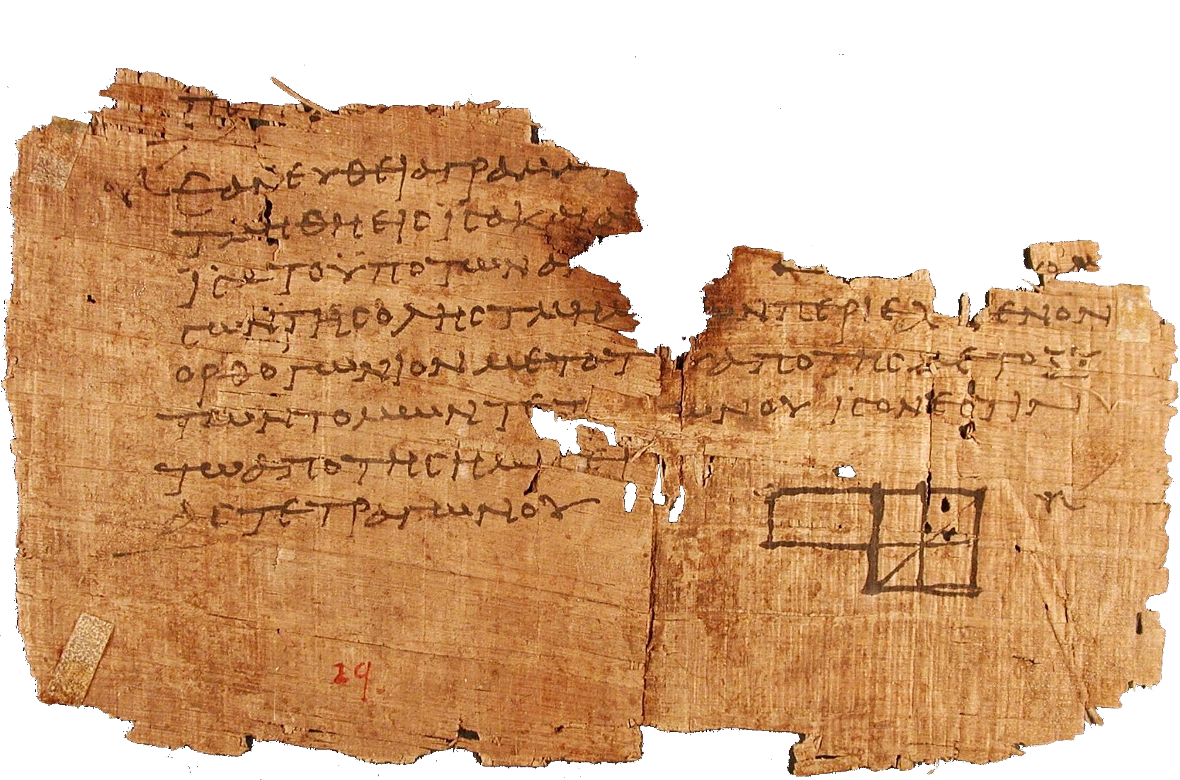
\includegraphics[width=\textwidth]{img/elements.png}}
	\only<2-4>{
	\only<2>{\centerline{Given a line $\ell$ and a point $P$, there exists}\centerline{\alert{one line through $P$ parallel to $\ell$.}}}
	\only<3>{\centerline{Given a line $\ell$ and a point $P$, there exists}\centerline{\alert{no line through $P$ parallel to $\ell$.}}}
	\only<4>{\centerline{Given a line $\ell$ and a point $P$, there exist}\centerline{\alert{at least two lines through $P$ parallel to $\ell$.}}}
	\vspace{\baselineskip}
	\begin{columns}[T,onlytextwidth]
	 \begin{column}{.33\textwidth}
	  \only<3>{
		\begin{alertbox}
		\centering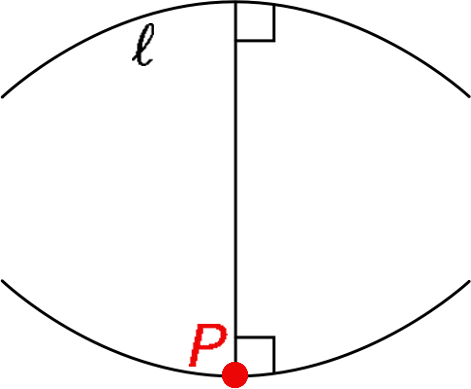
\includegraphics[width=\textwidth]{img/geo_elip.png}\\Elliptic
		\end{alertbox}
	  }
	  \only<4>{
		\begin{tbox}
		\centering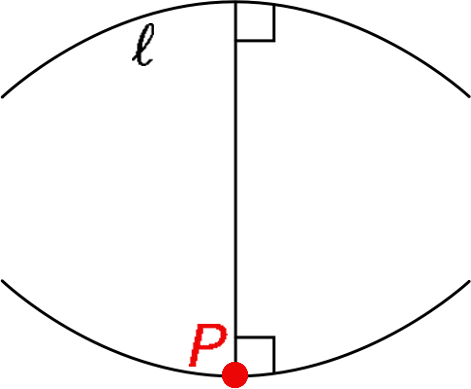
\includegraphics[width=\textwidth]{img/geo_elip.png}\\Elliptic
		\end{tbox}
	  }
	 \end{column}
	 \begin{column}{.34\textwidth}
	  \only<2>{
		\begin{alertbox}
			\centering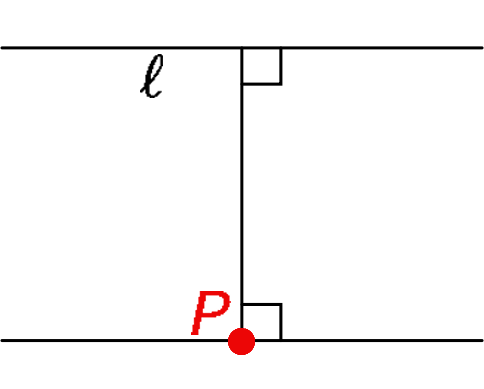
\includegraphics[width=\textwidth]{img/geo_eucl.png}\\Euclidean
		\end{alertbox}
	  }
	  \only<3-4>{
		\begin{tbox}
			\centering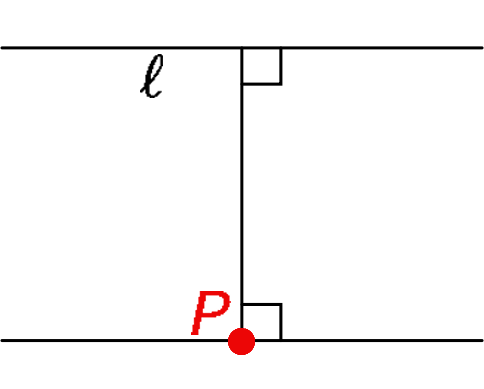
\includegraphics[width=\textwidth]{img/geo_eucl.png}\\Euclidean
		\end{tbox}
	  }
	 \end{column}
	 \begin{column}{.33\textwidth}
	  \only<4>{
		\begin{alertbox}
			\centering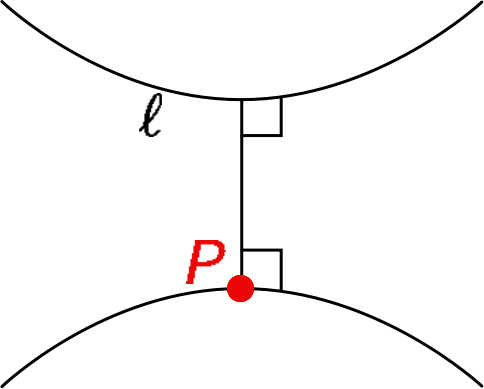
\includegraphics[width=\textwidth]{img/geo_hyp.png}\\Hyperbolic
		\end{alertbox}
	  }
	 \end{column}
	\end{columns}
	}
	\only<5->{
	\only<5>{\centerline{Given a line $\ell$ and a point $P$, there exist}\centerline{\alert{\textbf{?} many lines through $P$ parallel to $\ell$.}}}
	\only<6>{\centerline{\alert{Which axioms represent the truth?}}}
	\vspace{\baselineskip}
	\begin{alertbox}
	\begin{columns}[T,onlytextwidth]
	 \begin{column}{.33\textwidth}
		\centering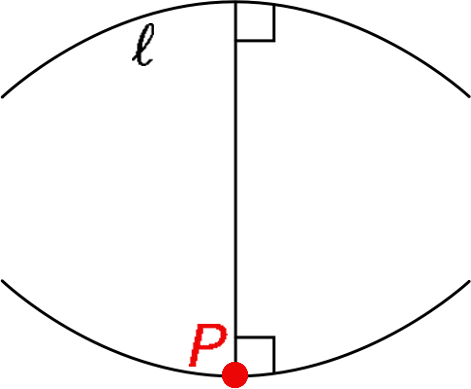
\includegraphics[width=0.73\textwidth]{img/geo_elip.png}\\Elliptic
	 \end{column}
	 \begin{column}{.34\textwidth}
		\centering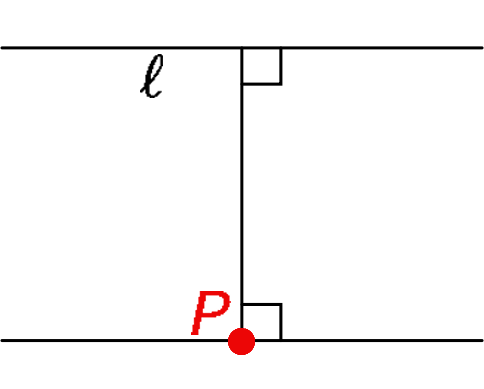
\includegraphics[width=0.73\textwidth]{img/geo_eucl.png}\\Euclidean
	 \end{column}
	 \begin{column}{.33\textwidth}
		\centering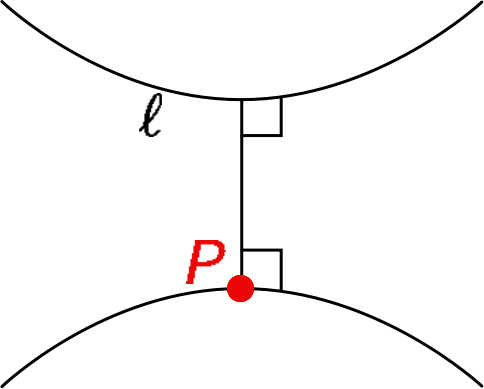
\includegraphics[width=0.73\textwidth]{img/geo_hyp.png}\\Hyperbolic
	 \end{column}
	\end{columns}
	\end{alertbox}
	}
\end{frame}
\begin{frame}{Search for Foundations}
	\begin{itemize}[<+->]
		\item Arithmetic of natural numbers by Peano
		\item Geometry by Hilbert and Pasch
		\item Predicate logic by Frege
	\end{itemize}
	\pause[\thebeamerpauses]
	\centering \alert{Desire for a universal and consistent system}
\end{frame}
\begin{frame}{Universal Systems}
    \begin{itemize}[<+->]
	\item Cantor's set theory
	\begin{itemize}
		\item \textit{``A set is a gathering together into a whole of definite, distinct objects of our perception or of our thought -- which are called elements of the set.''}\nocite{cantor_set}\hfill-- Georg Cantor
		\item Certainly universal, but informal and thus not adequate for a study of consistency
		\item Nonetheless, it was widely accepted.
	\end{itemize}
	\item Frege tried to build a consistent foundation by reducing mathematics to logic.
	\begin{itemize}
		\item<.-> Sophisticated work, but not well received
	\end{itemize}
	\item And then came Russell\ldots
    \end{itemize}
\end{frame}
\begin{frame}{Russell's Paradox}
	Consider \textit{the set of all sets that are not members of themselves}:
	\begin{equation*}
		R\coloneqq\{X\mid X\notin X\}
	\end{equation*}\pause
	Question: Is R a member of itself? That is, does $R\in R$ hold?\pause\\
	\vspace{\baselineskip}
	Answer:\hspace{4.3em}$R\in R \iff R\notin R$, a contradiction!
\end{frame}
\begin{frame}{The Begin of the Crisis}
    \begin{itemize}[<+->]
	\item Cantor's as well as Frege's system were victims of this paradox.
	\item \textit{``Hardly anything more unfortunate can befall a scientific writer than to have one of the foundations of his edifice shaken after the work is finished.''\nocite{frege_appendix}}\hfill-- Gottlob Frege
	\item Systems founded on Cantor's set theory were on shaky ground.
	\item A new foundation of mathematics had to be found.
    \end{itemize}
\end{frame}
%------------------------------------------------
\section{The Foundational Crisis}
\begin{frame}{The Three Schools of Thought}
    \begin{itemize}[<+->]
	\item Three schools of thought tried to establish a new foundation.
	\begin{itemize}
		\item<.-> Logicism
		\item<.-> Intuitionism
		\item<.-> Formalism
	\end{itemize}
    \end{itemize}
\centering{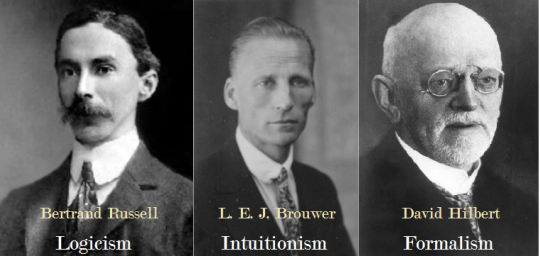
\includegraphics[height=0.42\textheight]{img/logic_intuit_form.png}\\
\scriptsize{Source: \url{geopolicraticus.tumblr.com/post/142561195372}}}
\end{frame}
%------------------------------------------------
\subsection{Logicism}
\begin{frame}{A Foundation Made of Logic}
    \begin{itemize}[<+->]
	\item Russell and Whitehead revisited Frege's idea of reducing mathematics to logic.	
	\item Mathematics is regarded as an extension of logic.
	\item Only fundamentally logical laws are used as axioms.
	\begin{itemize}
		\item Justifications that used axioms are self-evident truths
	\end{itemize}
	\item Chief work: Principia Mathematica
    \end{itemize}
\end{frame}
\begin{frame}{Principia Mathematica}
    \only<1-4>{
    \begin{itemize}[<+->]
	\item Type theory to avoid antinomies
	\item Difficulties in explaining some axioms
	\begin{itemize}
		\item<.-> Axiom of reducibility
		\item<.-> Axiom of infinity
	\end{itemize}
	\item Regarded as ``the outstanding example of an unreadable masterpiece''\nocite{math_experience}
	\item Nonetheless, many adopted it as a new foundation.
    \end{itemize}}
    \only<5>{
	    \begin{centering}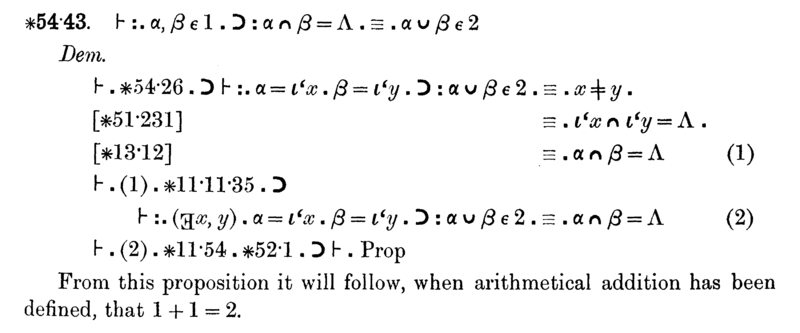
\includegraphics[width=\textwidth]{img/principia_mathematica.png}\end{centering}\\
	    \scriptsize{Principia Mathematica's infamous proof of $1+1=2$. It was not until page 379 that this proof was possible.}
    }
\end{frame}
%------------------------------------------------
\subsection{Intuitionism}
\begin{frame}{Proofs with Real Evidence}
    \begin{itemize}[<+->]
	\item Mathematics is \textbf{not} reducible to some formal system.
	\item Mathematics is a constructive process conducted by humans.
	\item The existence of any mathematical object is equivalent to the possibility of its construction, according to Brouwer.
	\begin{itemize}
		\item[$\Rightarrow$] No antinomies since paradoxical sets cannot be constructed
	\end{itemize}
	\item Consequently, some assumptions of classical logic must be rejected.
    \end{itemize}
\end{frame}
\begin{frame}{$P\lor\lnot P\equiv\ $?}
    \begin{itemize}[<+->]
	\item Intuitionists reject the \textit{law of excluded middle}: $\vdash P\lor\lnot P$\\
		\begin{centering}
			``For any proposition P, either P or its negation is true.''
		\end{centering}
    \end{itemize}
	\pause[\thebeamerpauses]
	\textbf{Proposition:} There exist two irrational numbers $a$ and $b$ such that $a^b$ is rational.\\\pause
	\vspace{\baselineskip}
	\textbf{Proof.} It is known that $\sqrt{2}$ is irrational. Let us consider the number $\sqrt{2}^{\sqrt{2}}$.\pause$ $ If it is rational, our statement is proved.\pause$ $ If it is irrational, $(\sqrt{2}^{\sqrt{2}})^{\sqrt{2}}=2$ proves our statement.\hfill$\qed$
\end{frame}
\begin{frame}{The Price to Pay}
    \begin{itemize}[<+->]
	\item Intuitionistic logic complicates many proofs.
	\item \textit{``Taking this tertium non datur (law of excluded middle) from the mathematician would be the same as, say, denying the astronomer his telescope and the boxer the use of his fists.''}\nocite{hilbert_tertium_non_datur}\\\hfill-- David Hilbert
	\item Consequently, only a few scholars adhered to intuitionism.
    \end{itemize}
\end{frame}
%------------------------------------------------
\subsection{Formalism}
\begin{frame}{Mathematics as a Symbolic Game}
    \begin{itemize}[<+->]
	\item Formalists support the autonomy of mathematics.
	\item Mathematics shall be based on symbols and axioms that describe syntactic operations on symbols.
	\item Mathematics does not need to justify the existence of its objects since its objects are just meaningless shapes.
    \end{itemize}
\end{frame}
\begin{frame}{Hilbert's Dream}
    \begin{itemize}[<+->]
	\item Hilbert feared the crippling effect of intuitionistic logic.
	\item To protect mathematics, he initiated a research programme called \textit{Hilbert's programme} that consists of two steps:
	\begin{enumerate}
		\item Formalise a system that is able to derive all of mathematics using syntactical operations
		\item Prove the system's consistency with metamathematical reasoning
	\end{enumerate}
	\item The dream of a complete and consistent mathematical system
    \end{itemize}
\end{frame}
%------------------------------------------------
\subsection{Peak and End}
\begin{frame}{The Peak of the Crisis}
    \begin{itemize}[<+->]
	\item In 1928, Brouwer boycotted the International Congress of Mathematicians.
	\item Hilbert presented his programme, without Brouwer being able to discredit his ideas.
	\item A few days after, Hilbert excluded Brouwer as a co-publisher from the journal ``Mathematischen Annalen''.
	\item Brouwer, in a state of frustration and despair, subsequently stopped publishing intuitionistic articles.
	\item Optimism for a complete and consistent formal system grew\ldots
    \end{itemize}
\end{frame}
\begin{frame}{The End of the Crisis}
\begin{columns}
 \begin{column}{.49\textwidth}
    \begin{itemize}[<+->]
	\item \ldots but then came Gödel.
	\item In 1931, he proved that there is no sufficiently strong, complete, and consistent formal system.
    \end{itemize}
 \end{column}
 \begin{column}{.49\textwidth}
  \centering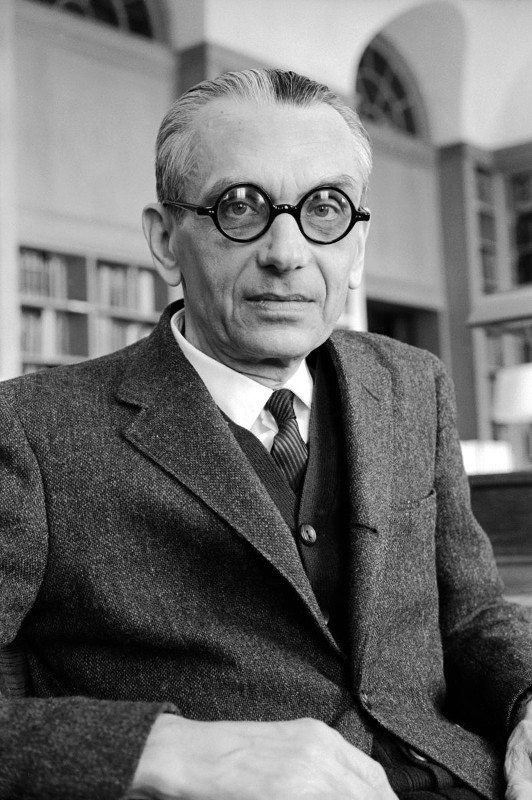
\includegraphics[height=0.3\textheight]{img/goedel.jpg}\\
		\scriptsize{Source: \url{newyorker.com/tech/elements/waiting-for-godel}}
 \end{column}
\end{columns}
	\visible<3->{\small{\begin{theorem}[First Incompleteness Theorem] Any consistent formal system rich enough to contain a formalisation of recursive arithmetic is incomplete.\end{theorem}}}
	\visible<4->{\small{\begin{theorem}[Second Incompleteness Theorem] Any consistent formal system rich enough to contain a formalisation of recursive arithmetic cannot prove its own consistency.\end{theorem}}}
\end{frame}
%------------------------------------------------
\section{Aftermath and Prospects}
\begin{frame}{Modern Mathematics}
    \begin{itemize}[<+->]
	\item To this day, formalism poses the foundation of mathematics.
	\begin{itemize}
		\item<.-> Zermelo-Fraenkel set theory (ZFC) as established foundation
	\end{itemize}
	\item Most modern mathematicians do not deal with foundational research but try to extend a specific branch of mathematics.
	\item The justification of foundations is often regarded philosophical work.
    \end{itemize}
\end{frame}
\begin{frame}{The Next Crisis?}
    \begin{itemize}[<+->]
	\item Digitisation of mathematics
	\item Can we trust proofs by computers?
	\item Some see it as an inevitable enrichment; others face it with distrust.
	\item Are we part of the next mathematical crisis?
    \end{itemize}
\end{frame}
%------------------------------------------------
%\section*{}
%------------------------------------------------
\begin{frame}
	\center
	\Large{Thanks for your attention! Any questions?}
	\vspace{0.5\baselineskip}\\
	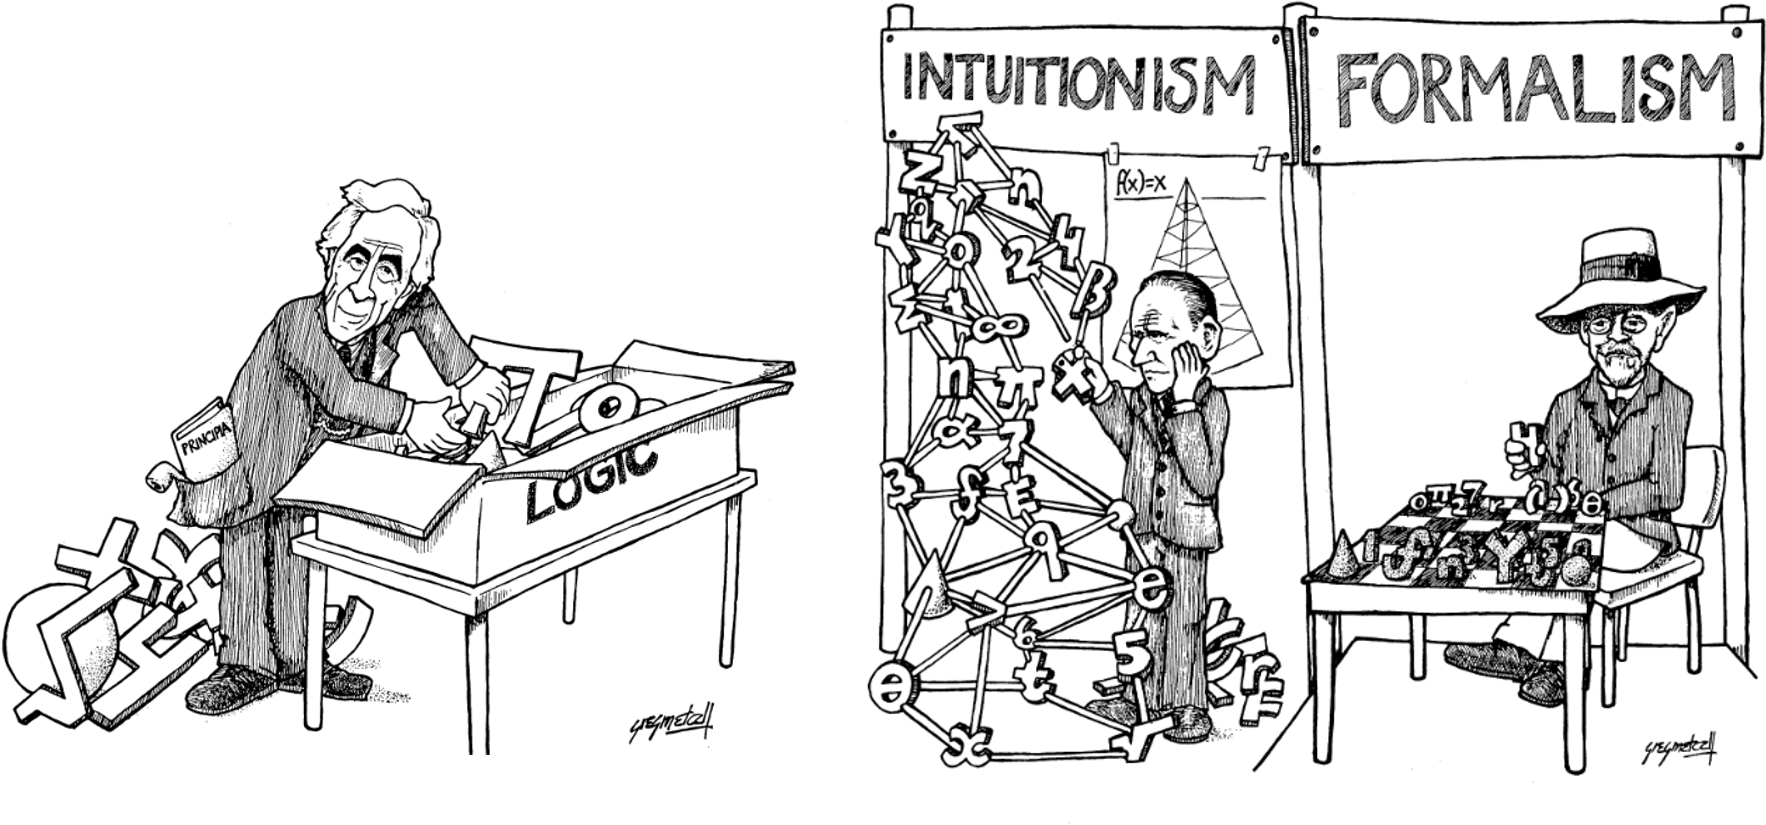
\includegraphics[height=0.6\textheight]{img/logic_intuit_form2.png}\\
	\scriptsize{Source: \url{maa.org/sites/default/files/pdf/upload\_library/22/Allendoerfer/1980/0025570x.di021111.02p0048m.pdf}}
\end{frame}
%----------------------------------------------------------------------------------------
\begin{frame}[allowframebreaks]{References}
  \bibliography{../paper/sources.bib}
  \bibliographystyle{abbrv}
\end{frame}

\begin{frame}[allowframebreaks]{Image sources}
\begin{itemize}
\item Euclid's Elements: \url{math.ubc.ca/~cass/Euclid/papyrus/tha.jpg}
\item Geometries: \url{upload.wikimedia.org/wikipedia/commons/thumb/7/78/Noneuclid.svg/2000px-Noneuclid.svg.png}
\end{itemize}
\end{frame}

\end{document} 
